\chapter{Quantum Software Engineering}
\label{cap:quantum}

\begin{inbreve}
I computer quantistici risolvono alcuni problemi molto più in fretta dei computer classici, ma oggi sono piccoli,
rumorosi e costosi. Il capitolo parte dai fondamenti: che cos'è un qubit, che cosa sono sovrapposizione ed
entanglement, come è fatto un computer quantistico e come lo si usa dal cloud. Poi spiega come si programma con i
circuiti quantistici e perché il risultato va stimato ripetendo l'esecuzione molte volte. Infine presenta la
\emph{Quantum Software Engineering} e tre sue tecniche per eseguire meglio i programmi quantistici. Le tecniche
distribuiscono l'esecuzione su più macchine, tagliano un circuito in frammenti, decidono quando smettere. Presuppone il
capitolo~\ref{cap:cloud}.
\end{inbreve}

\section{Perché il quantum computing}
\label{sec:qse-perche}

I computer quantistici possono risolvere diversi problemi \textbf{esponenzialmente più in fretta} dei computer
tradizionali. Per dirlo in modo preciso si usa una classe di complessità.

\begin{definizione}[BQP]
\termine{BQP} (\ingl{Bounded-error Quantum Polynomial time}) è la classe dei problemi di decisione che un computer
quantistico risolve in tempo polinomiale, con una probabilità di errore al massimo di $1/3$ su ogni istanza.
\end{definizione}

Un problema di decisione è un problema con risposta sì o no. \figrif{fig:qse-classi} colloca BQP rispetto alle classi
note. BQP contiene tutti i problemi P, cioè quelli risolvibili in tempo polinomiale da un computer classico. Contiene
anche alcuni problemi NP che non si sa risolvere in fretta con un computer classico.

\begin{figure}[ht]
\centering
\begin{tikzpicture}
\draw[rounded corners=6pt] (-3.2,-2.3) rectangle (3.2,2.3);
\node[font=\small] at (0,1.95) {PSPACE};
\draw[rounded corners=12pt, fill=blu!8] (-2.2,-1.7) rectangle (2.2,1.5);
\node[font=\small] at (0,1.15) {NP};
\draw[fill=rosso!12] (0,0.45) ellipse (1.2cm and 0.32cm);
\node[font=\footnotesize] at (0,0.45) {NP-complete};
\draw[fill=verde!15] (0,-0.9) ellipse (1.2cm and 0.32cm);
\node[font=\footnotesize] at (0,-0.9) {P};
\draw[rosso, dashed, thick] (0,-0.9) ellipse (2.9cm and 0.75cm);
\node[font=\footnotesize, text=rosso] at (2.72,-0.25) {BQP};
\end{tikzpicture}
\caption{Classi di complessità. PSPACE contiene NP, che contiene P e i problemi NP-complete. BQP (tratteggio rosso)
contiene P e parte di NP, ma non i problemi NP-complete, ed esce da NP.}
\label{fig:qse-classi}
\end{figure}

\tabrif{tab:qse-speedup} mostra due esempi di accelerazione.

\begin{table}[ht]
\centering
\small
\caption{Due problemi in cui un algoritmo quantistico batte il migliore algoritmo classico noto.}
\label{tab:qse-speedup}
\begin{tabularx}{\linewidth}{>{\raggedright\arraybackslash}p{2.6cm}>{\raggedright\arraybackslash}X>{\raggedright\arraybackslash}p{2.6cm}>{\raggedright\arraybackslash}p{4.4cm}}
\toprule
Problema & Spiegazione & Complessità quantistica & Complessità classica \\
\midrule
Fattorizzazione (Shor) & Scomporre un numero $N$ nel prodotto di interi più piccoli & polinomiale in $\log N$ &
  $\Theta\!\left(\exp\!\left(\left(\tfrac{32}{9}n\right)^{1/3}(\log n)^{2/3}\right)\right)$ \\
Ricerca (Grover) & Cercare un elemento in una sequenza di $n$ dati non ordinata & $O(\sqrt{n})$ & $O(n)$ \\
\bottomrule
\end{tabularx}
\end{table}

\subsubsection{Che cosa significa la tabella\aggiunta}
Per la ricerca, con $n = 1\,000\,000$ elementi un algoritmo classico deve guardarne fino a $1\,000\,000$, l'algoritmo di
Grover circa $\sqrt{10^6} = 1\,000$. Per la fattorizzazione il vantaggio è ancora più grande: il tempo classico cresce
quasi esponenzialmente con la dimensione del numero, quello quantistico solo in modo polinomiale. È per questo che la
fattorizzazione rapida minaccia la cifratura asimmetrica (\rif{sec:sic-cifratura}), la cui sicurezza si basa sulla
difficoltà di fattorizzare numeri grandi.

Le applicazioni attese sono molte. I tipi di problema in cui il quantum computing promette di più sono tre:
\textbf{simulazione}, \textbf{ottimizzazione} e \textbf{machine learning}. Da questi derivano applicazioni come
crittografia, chimica, scoperta di farmaci, materiali, logistica, previsioni meteo e climatiche, modelli finanziari,
e quindi settori come sanità, finanza, telecomunicazioni, trasporti ed energia.

\section{Che cos'è un computer quantistico}
\label{sec:qse-computer}

\begin{definizione}[Computer quantistico]
Un \termine{computer quantistico} è un dispositivo che sfrutta le proprietà della meccanica quantistica per eseguire
calcoli. Le due proprietà principali sono la \emph{sovrapposizione} (\ingl{superposition}) e l'\emph{entanglement}.
\end{definizione}

I \emph{qubit} sfruttano i principi della meccanica quantistica per offrire un nuovo modo di rappresentare ed elaborare
l'informazione. Per problemi specifici promettono vantaggi significativi rispetto al calcolo classico. Si passa
\emph{dai bit ai qubit}.

\subsection{Il qubit}
\label{sec:qse-qubit}

\begin{definizione}[Qubit]
\textbf{Concettualmente}, un \termine{qubit} è l'unità fondamentale dell'informazione quantistica. A differenza del bit
classico, il suo stato può essere ``0'', ``1'' oppure una \termine{sovrapposizione} (cioè una combinazione lineare) di
entrambi. Quando alla fine viene osservato, lo stato del qubit \textbf{collassa} su uno dei due stati semplici ``0'' o
``1'', con probabilità diverse che dipendono dalla sovrapposizione.

\textbf{Matematicamente}, un qubit è una combinazione lineare a coefficienti complessi dei suoi due stati di base:
``0'' (lo stato fondamentale, \ingl{ground state}) e ``1'' (lo stato eccitato, \ingl{excited state}):
\begin{equation}
\label{eq:qse-qubit}
\ket{\Psi} = \alpha\ket{0} + \beta\ket{1}.
\end{equation}
\end{definizione}

Nella \eqref{eq:qse-qubit}:
\begin{itemize}
  \item $\ket{\Psi}$ è il qubit;
  \item $\ket{0}$ e $\ket{1}$ sono i \termine{ket}, vettori a due dimensioni che rappresentano gli stati quantistici di
    base;
  \item $\alpha$ e $\beta$ sono le \termine{ampiezze}, numeri complessi che determinano le probabilità degli stati.
\end{itemize}

\subsubsection{Dalle ampiezze alle probabilità\aggiunta}
La probabilità di osservare ``0'' è $\abs{\alpha}^2$, quella di osservare ``1'' è $\abs{\beta}^2$. Le due probabilità
sommano a 1: $\abs{\alpha}^2 + \abs{\beta}^2 = 1$. Nell'esempio di \figrif{fig:qse-qubit} il qubit dà ``0'' con
probabilità $60\%$ e ``1'' con probabilità $40\%$: per esempio $\alpha = \sqrt{0{,}6} \approx 0{,}775$ e
$\beta = \sqrt{0{,}4} \approx 0{,}632$. I ket $\ket{0}$ e $\ket{1}$ si scrivono come i vettori $(1, 0)$ e $(0, 1)$,
quindi questo qubit è il vettore $(0{,}775;\ 0{,}632)$.

\begin{figure}[ht]
\centering
\begin{tikzpicture}
\node[draw, minimum size=1.0cm, font=\large] (q) at (0,0) {$\ket{\Psi}$};
\node[font=\Large] at (1.1,0) {$=$};
\node[font=\small] at (2.1,0) {$60\%$};
\node[circle, fill=blu, minimum size=0.7cm, text=white, font=\small] (z) at (3.1,0) {0};
\node[font=\small] at (4.5,0) {$40\%$};
\node[circle, fill=rosso, minimum size=0.7cm, text=white, font=\small] (u) at (5.5,0) {1};
\node[font=\footnotesize, anchor=north] at (0,-0.75) {qubit};
\node[font=\footnotesize, anchor=north, align=center] at (4.3,-0.75) {stati quantistici ($\ket{0}$, $\ket{1}$)\\con le loro probabilità};
\draw[->, thick] (7.0,0) -- node[above, font=\footnotesize] {misura} (8.6,0);
\node[circle, fill=blu, minimum size=0.7cm, text=white, font=\small] at (9.4,0.55) {0};
\node[font=\footnotesize, anchor=west] at (9.9,0.55) {con prob.\ $0{,}6$};
\node[circle, fill=rosso, minimum size=0.7cm, text=white, font=\small] at (9.4,-0.55) {1};
\node[font=\footnotesize, anchor=west] at (9.9,-0.55) {con prob.\ $0{,}4$};
\end{tikzpicture}
\caption{Un qubit in sovrapposizione: stato ``0'' con probabilità $60\%$ (blu) e stato ``1'' con probabilità $40\%$
(rosso). Quando lo si misura collassa su uno solo dei due stati.}
\label{fig:qse-qubit}
\end{figure}

\subsection{Entanglement}
\label{sec:qse-entanglement}

\begin{definizione}[Entanglement]
Più qubit possono essere \termine{entangled}: lo stato di un qubit diventa direttamente correlato allo stato di un
altro, per quanto lontani siano.
\end{definizione}

Per esempio due qubit entangled possono trovarsi al $50\%$ nello stato ``blu-rosso'' e al $50\%$ nello stato
``rosso-blu''. Presi da soli, i due qubit sono imprevedibili. Insieme però sono legati: se misurando il primo si ottiene
blu, il secondo è sicuramente rosso, e viceversa.

\subsection{Come è fatto}
\label{sec:qse-hardware}

Un computer quantistico a superconduttori ha cinque parti (\figrif{fig:qse-hardware}).
\begin{description}[leftmargin=0pt, style=unboxed]
  \item[Quantum processor.] Il processore quantistico, in fondo al refrigeratore, contiene i qubit.
  \item[Dilution refrigerator.] Il refrigeratore a diluizione: la struttura a piani che raffredda il processore a
    temperature bassissime.
  \item[Enclosure.] L'involucro che chiude il refrigeratore.
  \item[Measurement interface.] L'interfaccia di misura che legge lo stato dei qubit.
  \item[Classical controller.] Un normale computer che controlla il processore. Scrive le istruzioni verso il
    processore (\ingl{electronic writing}) e ne legge i risultati (\ingl{electronic reading}). Sul controller si
    programma con kit di sviluppo come \emph{Qiskit} e \emph{Cirq}.
\end{description}

\begin{figure}[ht]
\centering
\begin{tikzpicture}
\draw[rounded corners=4pt, fill=grigiochiaro] (0,-2.2) rectangle (2.6,2.2);
\node[font=\footnotesize, anchor=north] at (1.3,-2.25) {Enclosure};
\foreach \y in {1.6,0.9,0.2,-0.5} \draw[arancio, thick] (0.3,\y) -- (2.3,\y);
\draw[arancio] (0.5,1.6) -- (0.5,-1.2) (2.1,1.6) -- (2.1,-1.2);
\node[font=\scriptsize, align=center] at (1.3,1.25) {dilution\\refrigerator};
\node[draw, fill=white, font=\scriptsize, align=center] (qp) at (1.3,-1.45) {quantum\\processor};
\node[draw, fill=white, font=\scriptsize, align=center] (mi) at (4.2,-1.45) {measurement\\interface};
\draw (qp) -- (mi);
\node[blocco, align=center] (cc) at (9.0,0) {Classical controller\\{\footnotesize Qiskit, Cirq}};
\draw[->, thick, blu] (cc.west |- 0,0.5) -- node[above, font=\footnotesize] {electronic writing} (2.6,0.5);
\draw[->, thick, verde] (mi.east) -| node[pos=0.25, below, font=\footnotesize] {electronic reading} ([xshift=-6mm]cc.south);
\end{tikzpicture}
\caption{Le parti di un computer quantistico. Il controller classico scrive le istruzioni verso il processore
quantistico, che sta in fondo al refrigeratore a diluizione dentro l'involucro. L'interfaccia di misura legge lo stato
dei qubit e lo rimanda al controller.}
\label{fig:qse-hardware}
\end{figure}

Negli ultimi trent'anni la tecnologia è progredita molto. Si è passati dai 2 qubit di fine anni Novanta ai processori
con centinaia o migliaia di qubit di oggi, come i 1\,121 qubit di IBM. I computer quantistici cominciano a essere
largamente disponibili.

\subsection{Le tecnologie dei qubit}
\label{sec:qse-tecnologie}

Esistono diverse tecnologie per realizzare un qubit: ``scegli il qubit e trovi le caratteristiche''
(\tabrif{tab:qse-tecnologie}). Le caratteristiche che le distinguono sono:
\begin{itemize}
  \item il \emph{qubit lifetime}, il record di tempo di coerenza di un qubit, cioè per quanto mantiene il suo stato;
  \item la \emph{gate fidelity}, la più alta fedeltà riportata per un'operazione su due qubit;
  \item il \emph{gate operation time}, la velocità di un'operazione;
  \item la \emph{connectivity}, cioè quali qubit possono interagire tra loro;
  \item la \emph{scalability}, cioè quanto è facile aumentare il numero di qubit.
\end{itemize}

\begin{table}[ht]
\centering
\footnotesize
\caption{Tecnologie dei qubit. Valori indicativi (``c.'' = circa); s = secondi, $\mu$s = $10^{-6}$ s, ns = $10^{-9}$ s.
TBC = da confermare.}
\label{tab:qse-tecnologie}
\begin{tabularx}{\linewidth}{>{\raggedright\arraybackslash}p{1.75cm}>{\raggedright\arraybackslash}p{1.8cm}>{\raggedright\arraybackslash}p{1.25cm}>{\raggedright\arraybackslash}p{1.05cm}>{\raggedright\arraybackslash}p{1.1cm}>{\raggedright\arraybackslash}p{1.15cm}>{\raggedright\arraybackslash}X}
\toprule
Tecnologia & Esempi & Lifetime & Fidelity & Gate time & Connes\-sioni & Pro e contro \\
\midrule
Supercon\-ducting & IBM, Google, Rigetti, Alibaba, Intel & c.\ 50--100 $\mu$s & c.\ 99,4\% & c.\ 10--50 ns & vicini &
  + operazioni veloci, sfrutta l'industria dei semiconduttori, molto scalabile; $-$ vita breve, va tenuto molto freddo \\
Ion trap & IonQ, AQT, Honeywell & oltre 1\,000 s & c.\ 99,9\% & c.\ 3--50 $\mu$s & tutti con tutti &
  + alta fedeltà, molto stabile; $-$ operazioni lente \\
Photonics & PsiQuantum, Xanadu & c.\ 150 $\mu$s & c.\ 98,0\% & c.\ 1 ns & non nota &
  + molto scalabile, nessun requisito di temperatura; $-$ tecnologia nascente, connettività da dimostrare \\
Neutral atoms & Atom Computing, PASQAL, QuEra & simile allo ion trap & c.\ 95\% & TBC & TBC &
  + lunghi tempi di coerenza; $-$ va tenuto freddo, nascente \\
Silicon & Intel, Silicon Quantum Computing & c.\ 1--10 s & c.\ 99\% & c.\ 1--10 ns & vicini &
  + stabile, sfrutta l'industria dei semiconduttori; $-$ va tenuto freddo, nascente \\
Topological & Microsoft (in sviluppo) & molto alta (stima) & molto alta (stima) & non nota & non nota &
  + vita lunga e alta fedeltà stimate; $-$ esistenza da confermare \\
\bottomrule
\end{tabularx}
\end{table}

\subsection{Topologie}
\label{sec:qse-topologie}

Per eseguire un'operazione su più qubit, i qubit coinvolti devono essere collegati ``fisicamente''. I modi di
collegare i qubit si chiamano \termine{topologie} (\figrif{fig:qse-topologie}). Ogni processore ha la propria.

\begin{figure}[ht]
\centering
\begin{tikzpicture}[q/.style={circle, fill=blu!70, minimum size=5pt, inner sep=0pt}]
% linea
\foreach \i in {0,...,6} \node[q] (a\i) at (0.45*\i,0) {};
\foreach \i [evaluate=\i as \j using int(\i+1)] in {0,...,5} \draw[blu!70] (a\i) -- (a\j);
\node[font=\footnotesize] at (1.35,-0.9) {linea};
% scala
\begin{scope}[xshift=4cm]
\foreach \i in {0,...,5} { \node[q] (b\i) at (0.45*\i,0.3) {}; \node[q] (c\i) at (0.45*\i,-0.3) {}; \draw[blu!70] (b\i) -- (c\i); }
\foreach \i [evaluate=\i as \j using int(\i+1)] in {0,...,4} \draw[blu!70] (b\i) -- (b\j) (c\i) -- (c\j);
\node[font=\footnotesize] at (1.12,-0.9) {scala};
\end{scope}
% griglia
\begin{scope}[xshift=8cm, yshift=-0.6cm]
\draw[blu!70, step=0.4] (0,0) grid (1.2,1.2);
\foreach \x in {0,...,3} \foreach \y in {0,...,3} \node[q] at (0.4*\x,0.4*\y) {};
\node[font=\footnotesize] at (0.6,-0.3) {griglia};
\end{scope}
\end{tikzpicture}
\caption{Tre topologie schematiche. Ogni punto è un qubit, ogni segmento un collegamento fisico. Un'operazione su due
qubit si fa direttamente solo tra qubit collegati: in una linea ogni qubit ha al più due vicini, in una griglia fino a
quattro.}
\label{fig:qse-topologie}
\end{figure}

\subsection{Come si accede a un computer quantistico}
\label{sec:qse-accesso}

Un computer quantistico è grande, costoso e va tenuto a temperature bassissime: non si compra. Vi si accede con il
\textbf{cloud computing} (capitolo~\ref{cap:cloud}). Molti fornitori offrono accesso ai propri computer quantistici.
Tra questi IBM Quantum, Google Quantum AI, Amazon Braket, Microsoft Azure Quantum, Xanadu, D-Wave, Rigetti, AQT,
Oxford Quantum Circuits (OQC) e Quantum Inspire. Ogni fornitore elenca le macchine disponibili con le loro
caratteristiche:
\begin{itemize}
  \item numero di qubit;
  \item stato (\emph{online}, coda in pausa, riservata);
  \item lunghezza della coda di lavori in attesa;
  \item tipo di processore;
  \item tipo di piano (aperto o a pagamento).
\end{itemize}

\section{Programmare un computer quantistico}
\label{sec:qse-programmare}

Un computer quantistico si programma con i \termine{circuiti quantistici}. Un circuito è una sequenza di \emph{porte}
(\ingl{gate}), operazioni elementari sui qubit, seguita dalle misure.

\begin{esempio}[Un circuito in OpenQASM]
Il programma seguente, scritto in OpenQASM 2.0, prepara due qubit entangled e li misura.
\begin{verbatim}
1  OPENQASM 2.0;
2  include "qelib1.inc";
3
4  qreg q1[1];
5  qreg q2[1];
6  creg q1c[1];
7  creg q2c[1];
8
9  h q1[0];
10 cx q1[0],q2[0];
11 measure q1[0] -> q1c[0];
12 measure q2[0] -> q2c[0];
\end{verbatim}
\begin{itemize}
  \item Righe 4--7: due registri quantistici di un qubit (\texttt{qreg}) e due registri classici di un bit
    (\texttt{creg}), che riceveranno i risultati delle misure. Lo stato iniziale dei due qubit è \texttt{00}.
  \item Riga 9: la porta \texttt{h} (Hadamard) mette \texttt{q1} in sovrapposizione. Lo stato diventa \texttt{00} al
    $50\%$ e \texttt{01} al $50\%$.
  \item Riga 10: la porta \texttt{cx} (CNOT) inverte \texttt{q2} se \texttt{q1} vale 1. I due qubit diventano
    entangled: lo stato è \texttt{00} al $50\%$ e \texttt{11} al $50\%$.
  \item Righe 11--12: le misure copiano i qubit nei bit classici. Il risultato è \texttt{00} oppure \texttt{11}.
\end{itemize}
\end{esempio}

\begin{figure}[ht]
\centering
\begin{tikzpicture}
\node[font=\small, anchor=east] at (0,0) {$q1_0$};
\node[font=\small, anchor=east] at (0,-1) {$q2_0$};
\node[font=\small, anchor=east] at (0,-2) {$q1c_0$};
\node[font=\small, anchor=east] at (0,-2.8) {$q2c_0$};
\draw (0,0) -- (6.2,0);
\draw (0,-1) -- (6.2,-1);
\draw[double, double distance=1.5pt] (0,-2) -- (6.2,-2);
\draw[double, double distance=1.5pt] (0,-2.8) -- (6.2,-2.8);
\node[draw, fill=blu!20, minimum size=0.6cm, font=\small] at (1.1,0) {H};
\fill (2.4,0) circle (2.5pt);
\draw (2.4,0) -- (2.4,-1.25);
\draw[fill=white] (2.4,-1) circle (0.25cm);
\draw (2.15,-1) -- (2.65,-1) (2.4,-0.75) -- (2.4,-1.25);
\node[draw, fill=grigiochiaro, minimum size=0.6cm, font=\scriptsize] (m1) at (3.8,0) {M};
\node[draw, fill=grigiochiaro, minimum size=0.6cm, font=\scriptsize] (m2) at (5.1,-1) {M};
\draw[->, double, double distance=1pt] (m1.south) -- (3.8,-1.9);
\draw[->, double, double distance=1pt] (m2.south) -- (5.1,-2.7);
\node[font=\scriptsize, anchor=north east] at (0,-3.1) {stato:};
\node[font=\scriptsize, anchor=north] at (0.45,-3.1) {00};
\node[font=\scriptsize, align=center, anchor=north] at (1.75,-3.1) {50\% 00\\50\% 01};
\node[font=\scriptsize, align=center, anchor=north] at (3.1,-3.1) {50\% 00\\50\% 11};
\node[font=\scriptsize, align=center, anchor=north] at (5.1,-3.1) {00 oppure\\11};
\begin{axis}[stile, at={(8.1cm,-3.0cm)}, width=5.4cm, height=4.4cm, ybar, bar width=10pt, ymin=0, ymax=100,
  enlarge x limits=0.2,
  xtick=data, symbolic x coords={00,01,10,11}, ylabel={probabilità (\%)}, ylabel style={font=\footnotesize},
  xlabel={stati prima della misura}, xlabel style={font=\footnotesize}]
\addplot[fill=blu!50, draw=blu] coordinates {(00,50) (01,0) (10,0) (11,50)};
\end{axis}
\end{tikzpicture}
\caption{Il circuito dell'esempio e il suo risultato. A sinistra le righe dei due qubit (singole) e dei due bit
classici (doppie): porta H su \texttt{q1}, porta CNOT con controllo su \texttt{q1} (punto) e bersaglio su \texttt{q2}
($\oplus$), due misure (M). Sotto, lo stato dopo ogni passo. A destra la distribuzione degli stati prima della misura:
\texttt{00} e \texttt{11} al $50\%$ ciascuno.}
\label{fig:qse-circuito}
\end{figure}

\subsection{Il risultato è probabilistico}
\label{sec:qse-shot}

\begin{idea}[Perché servono molti shot]
\begin{enumerate}
  \item Dopo l'esecuzione di un circuito quantistico lo stato quantistico è di solito in \textbf{sovrapposizione} di più
    stati finali (per esempio $60\%$ ``0'' e $40\%$ ``1'').
  \item Le leggi della fisica impediscono di \textbf{osservare direttamente} lo stato quantistico.
  \item Si può solo \textbf{misurarlo}. Quando lo si misura, lo stato \textbf{collassa} su un unico stato di uscita.
  \item Quindi si esegue lo stesso circuito, con lo stesso input, molte volte. Ogni esecuzione si chiama
    \termine{shot}. Le frequenze dei risultati degli shot \textbf{approssimano} la vera distribuzione dello stato
    quantistico.
\end{enumerate}
\end{idea}

\begin{esempio}[Stimare il $60\%$ e il $40\%$\aggiunta]
Il qubit di \figrif{fig:qse-qubit} si esegue e si misura 10 volte. Si ottiene per esempio 0, 1, 0, 0, 1, 0, 0, 1, 0, 0:
sette ``0'' e tre ``1'', cioè $70\%$ e $30\%$. Con 10 shot la stima è ancora lontana dal $60\%$--$40\%$. Più shot si
eseguono, più le frequenze si avvicinano alle probabilità vere. Il prezzo è che ogni shot costa tempo e denaro.
\end{esempio}

\subsection{L'era NISQ}
\label{sec:qse-nisq}

I dispositivi attuali sono detti \termine{NISQ} (\ingl{Noisy Intermediate-Scale Quantum}).
\begin{itemize}
  \item Sono molto sensibili alle interferenze esterne, il \termine{rumore} (\ingl{noise}).
  \item Non riescono ad aumentare facilmente la propria dimensione, cioè il numero di qubit.
\end{itemize}
Di conseguenza eseguono solo programmi quantistici con pochi qubit e pochi passi consecutivi. \uline{I programmi più
lunghi sarebbero molto influenzati dal rumore.} Oggi si possono eseguire solo circuiti piccoli.

\section{Quantum Software Engineering}
\label{sec:qse-qse}

I computer quantistici disponibili hanno ancora dei limiti:
\begin{itemize}
  \item \textbf{affidabilità}: i tassi di errore sono alti;
  \item \textbf{scalabilità}: il numero di qubit è limitato;
  \item \textbf{costo}.
\end{itemize}
Anche lo sviluppo del software quantistico ha dei limiti:
\begin{itemize}
  \item si programma ancora soprattutto combinando porte di basso livello in circuiti;
  \item l'interoperabilità tra software e macchine è limitata;
  \item c'è poco supporto per l'intero ciclo di vita del software.
\end{itemize}
Chi sviluppa software quantistico (sviluppatori, operatori, ricercatori) non ha ancora l'insieme di strumenti che il
software classico ha: container, orchestratori, pipeline di integrazione continua, strumenti di monitoraggio
(capitoli~\ref{cap:kubernetes}--\ref{cap:devops}).

\begin{definizione}[Quantum Software Engineering]
La \termine{Quantum Software Engineering} (QSE) è ``l'uso di solidi principi di ingegneria per lo sviluppo, l'esercizio
e la manutenzione del software quantistico e della documentazione associata, per ottenere in modo economico software
quantistico affidabile e che funzioni in modo efficiente sui computer quantistici'' (Zhao, 2020).
\end{definizione}

Il \termine{Talavera Manifesto} (M.~Piattini et al., 2020) elenca che cosa la QSE dovrebbe fare:
\begin{enumerate}
  \item essere indipendente dai linguaggi di programmazione e dalle tecnologie quantistiche;
  \item accettare la coesistenza di calcolo classico e quantistico;
  \item sostenere la gestione dei progetti di sviluppo di software quantistico;
  \item considerare l'evoluzione del software quantistico;
  \item puntare a programmi quantistici con, auspicabilmente, zero difetti;
  \item garantire la qualità del software quantistico;
  \item promuovere il riuso del software quantistico;
  \item affrontare sicurezza e privacy fin dalla progettazione (\ingl{by design});
  \item coprire la governance e la gestione del software.
\end{enumerate}

Esempi di obiettivi della QSE sono:
\begin{itemize}
  \item migliorare i \emph{transpiler}, i programmi che traducono un circuito nelle porte e nella topologia di una
    macchina specifica;
  \item rendere il codice riusabile, per esempio con modelli di moduli quantistici (\ingl{Q module template});
  \item rendere possibile la verifica dei programmi, per esempio dimostrare che due programmi $P$ e $Q$ sono
    equivalenti;
  \item rendere possibile la coesistenza di calcolo classico e quantistico, come in $x = f(y) \oplus q(z)$, dove $f$ è
    una parte classica e $q$ una parte quantistica;
  \item sfruttare meglio computer quantistici eterogenei e inaffidabili.
\end{itemize}
Le tre sezioni che seguono sono esempi dell'ultimo obiettivo.

\section{Distribuire gli shot su più macchine}
\label{sec:qse-shotwise}

\subsection{Motivazioni}

Le QPU attuali (\ingl{Quantum Processing Units}, i processori quantistici) hanno due limiti:
\begin{itemize}
  \item pochi qubit;
  \item alta sensibilità al rumore, per cui bisogna eseguire migliaia di shot (\rif{sec:qse-shot}).
\end{itemize}
La domanda di solito è: \emph{su quale QPU conviene eseguire l'algoritmo?} La domanda di questa sezione è un'altra:
\emph{perché sceglierne una sola?} Si possono sfruttare la sensibilità al rumore e l'eterogeneità delle QPU attuali?

\subsection{L'idea: split e merge}

\begin{definizione}[Shot-wise distribution]
Con la \termine{shot-wise distribution} si \textbf{dividono} (\ingl{split}) gli shot di un calcolo quantistico tra più
QPU. Poi si \textbf{fondono} (\ingl{merge}) le distribuzioni parziali prodotte da ogni QPU per ottenere la
distribuzione finale (\figrif{fig:qse-split}).
\end{definizione}

\begin{figure}[ht]
\centering
\begin{tikzpicture}[qpu/.style={draw, rounded corners=2pt, minimum width=1.2cm, minimum height=0.8cm, font=\footnotesize}]
\node[blocco, align=center] (c) at (0,0) {circuito\\$s$ shot};
\node[qpu, fill=white] (p1) at (3.6,1.4) {QPU 1};
\node[qpu, fill=verde!25] (p2) at (3.6,0) {QPU 2};
\node[qpu, fill=inchiostro, text=white] (p3) at (3.6,-1.4) {QPU 3};
\foreach \p in {p1,p2,p3} \draw[->] (c.east) -- node[above, sloped, font=\scriptsize] {$s/3$} (\p.west);
\foreach \p/\y/\h in {p1/1.4/{0.20,0.30,0.35,0.15}, p2/0/{0.15,0.35,0.30,0.20}, p3/-1.4/{0.25,0.25,0.40,0.10}} {
  \foreach \v [count=\k] in \h \fill[grigio] (5.0+0.25*\k,\y-0.4) rectangle ++(0.18,\v*2.2);
  \draw[->] (\p.east) -- (5.15,\y);
}
\foreach \y in {1.4,0,-1.4} \draw[->] (6.4,\y) -- (7.6,0);
\foreach \v [count=\k] in {0.20,0.30,0.35,0.15} \fill[verde] (7.8+0.3*\k,-0.4) rectangle ++(0.22,\v*2.2);
\draw[decorate, decoration={brace, mirror, amplitude=5pt}] (0.9,-2.1) -- (4.3,-2.1) node[midway, below=5pt, font=\footnotesize] {split};
\draw[decorate, decoration={brace, mirror, amplitude=5pt}] (5.1,-2.1) -- (9.2,-2.1) node[midway, below=5pt, font=\footnotesize] {merge};
\end{tikzpicture}
\caption{Split e merge uniformi. Gli $s$ shot del circuito sono divisi in tre parti uguali, $s/3$ per QPU. Ogni QPU
produce una distribuzione parziale (istogrammi grigi), diversa per il rumore della macchina. Le tre distribuzioni sono
fuse nella distribuzione finale (verde). Le altezze sono qualitative.}
\label{fig:qse-split}
\end{figure}

Le \textbf{politiche} per dividere (e fondere) sono molte, per esempio:
\begin{itemize}
  \item \emph{uniform}: gli shot sono divisi in parti uguali tra tutte le QPU disponibili;
  \item \emph{random}: gli shot sono divisi a caso;
  \item \emph{time-aware}: si tiene conto dei tempi delle QPU;
  \item \emph{noise-aware}: si tiene conto del rumore di ogni QPU.
\end{itemize}

\begin{esempio}[Merge uniforme\aggiunta]
Con $s = 3\,000$ shot e tre QPU, ognuna esegue $1\,000$ shot. Si supponga che lo stato \texttt{011} esca 210 volte sulla
prima QPU, 190 sulla seconda e 240 sulla terza (numeri di esempio). Con il merge uniforme le frequenze si sommano:
$(210 + 190 + 240)/3\,000 = 640/3\,000 \approx 21{,}3\%$. Una QPU particolarmente rumorosa sposta il risultato meno di
quanto lo sposterebbe se si usasse solo lei.
\end{esempio}

\subsection{Funziona davvero?}

Negli esperimenti si sono provate 3 politiche di split per 3 politiche di merge, cioè 9 combinazioni.
\begin{itemize}
  \item \textbf{Uniform}: shot divisi in parti uguali tra tutte le QPU disponibili.
  \item Due politiche \textbf{noise-aware}. Prima c'è una \emph{fase di calibrazione}: si esegue su ogni QPU un insieme
    di circuiti di addestramento e si confrontano i risultati con quelli di un simulatore esatto. Così si stima
    l'affidabilità di ogni QPU.
    \begin{itemize}
      \item \textbf{Hellinger}: gli shot sono divisi in modo da minimizzare la distanza di Hellinger totale (al
        quadrato) dei risultati attesi delle QPU. La distanza di Hellinger misura quanto due distribuzioni di
        probabilità sono diverse.
      \item \textbf{MISE}: gli shot sono divisi tenendo conto anche degli errori statistici attesi (minimo
        \ingl{Mean Integrated Square Error}).
    \end{itemize}
\end{itemize}
Gli esperimenti sono stati eseguiti su 7 QPU di IBM e IonQ.

\subsubsection{Risultati quantitativi}
I risultati misurano l'errore rispetto alla distribuzione esatta, al variare del numero di QPU (da 2 a 7).
\begin{itemize}
  \item I risultati \emph{non} superano quelli della migliore QPU presa da sola, ma spesso superano quelli di una
    singola QPU.
  \item Al crescere del numero di QPU l'errore massimo diminuisce.
  \item L'errore medio resta paragonabile a quello dell'esecuzione su una sola QPU.
  \item La deviazione standard dei risultati si riduce.
\end{itemize}

\subsubsection{Risultati qualitativi}
\begin{itemize}
  \item[$+$] \textbf{Robustezza al rumore quantistico}: l'impatto dell'errore si riduce, i risultati sono più stabili e
    il caso peggiore migliora.
  \item[$+$] \textbf{Bilanciamento del carico} tra le QPU.
  \item[$+$] \textbf{Resilienza ai guasti delle QPU}: se una QPU non risponde, le altre continuano.
  \item[$+$] \textbf{Riduzione dei tempi di attesa} nelle code.
\end{itemize}

\subsubsection{Osservazioni}
Le sfide sono due:
\begin{itemize}
  \item la distribuzione degli shot può \emph{diluire} le prestazioni del caso migliore, cioè della QPU migliore;
  \item le politiche noise-aware dipendono dall'accuratezza e dalla frequenza delle calibrazioni delle QPU.
\end{itemize}
\uline{Conclusione complessiva: la shot-wise distribution conviene.} Le estensioni possibili sono:
\begin{itemize}
  \item studiare meglio la mitigazione degli errori a livello di shot;
  \item considerare altre politiche di split e merge (\rif{sec:qse-cut});
  \item sviluppare calibrazioni adatte a scenari specifici;
  \item studiare esecuzioni incrementali, per ridurre il numero di shot (\rif{sec:qse-stop}).
\end{itemize}

\subsection{Quantum Broker}

Il \termine{Quantum Broker} è il prototipo di un servizio che esegue distribuzioni shot-wise su insiemi di QPU, tenendo
conto dei requisiti dell'utente (\figrif{fig:qse-broker}). L'utente invia il circuito e i requisiti di qualità del
servizio (\ingl{QoS requirements}) e riceve i risultati fusi. I requisiti si esprimono come vincoli e obiettivo.

\begin{esempio}[Requisiti per il Quantum Broker]
\begin{verbatim}
constraints:
    max(execution_time + waiting_time) <= 1700
    min(fidelity) >= 0.85
    sum(cost) <= 750
objective:
    -sum(cost)
\end{verbatim}
Il tempo di esecuzione più quello di attesa non deve superare 1\,700, la fedeltà di ogni QPU usata deve essere almeno
$0{,}85$ e il costo totale al massimo 750. Tra le distribuzioni che rispettano i vincoli si sceglie quella che
massimizza $-\text{costo}$, cioè quella che costa meno.
\begin{verbatim}
constraints:
    shots['fake_torino'] >= 700
    sum(cost) <= 700
objective:
    max(execution_time + waiting_time)
\end{verbatim}
Almeno 700 shot vanno sulla macchina \texttt{fake\_torino} e il costo totale non supera 700. L'obiettivo è il tempo
massimo di esecuzione più attesa.
\end{esempio}

\begin{figure}[ht]
\centering
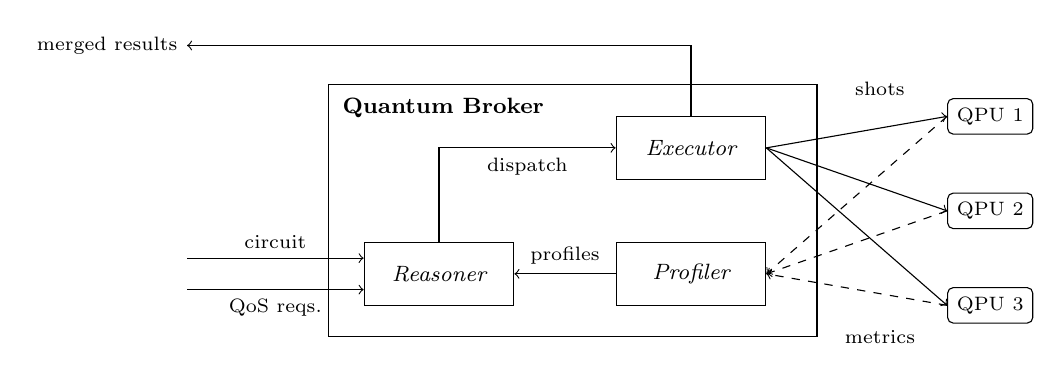
\begin{tikzpicture}[b/.style={draw, minimum width=1.9cm, minimum height=0.8cm, font=\footnotesize\itshape}]
\draw (0,-1.6) rectangle (6.2,1.6);
\node[font=\footnotesize\bfseries, anchor=north west] at (0.05,1.55) {Quantum Broker};
\node[b] (r) at (1.4,-0.8) {Reasoner};
\node[b] (p) at (4.6,-0.8) {Profiler};
\node[b] (e) at (4.6,0.8) {Executor};
\draw[->] (p) -- node[above, font=\scriptsize] {profiles} (r);
\draw[->] (r.north) |- node[pos=0.75, below, font=\scriptsize] {dispatch} (e.west);
\foreach \y/\n in {1.2/1, 0/2, -1.2/3} \node[draw, rounded corners=2pt, font=\scriptsize] (q\n) at (8.4,\y) {QPU \n};
\foreach \n in {1,2,3} { \draw[->] (e.east) -- (q\n.west); \draw[->, dashed] (q\n.west) -- (p.east); }
\node[font=\scriptsize] at (7.0,1.55) {shots};
\node[font=\scriptsize] at (7.0,-1.6) {metrics};
\draw[->] (-1.8,-0.6) -- node[above, font=\scriptsize] {circuit} (r.west |- 0,-0.6);
\draw[->] (-1.8,-1.0) -- node[below, font=\scriptsize] {QoS reqs.} (r.west |- 0,-1.0);
\draw[->] (e.north) |- (-1.8,2.1) node[left, font=\scriptsize] {merged results};
\end{tikzpicture}
\caption{Architettura del Quantum Broker. Il Reasoner riceve circuito e requisiti QoS e, con i profili delle QPU
forniti dal Profiler, decide la divisione degli shot. L'Executor invia gli shot alle QPU e restituisce i risultati fusi.
Il Profiler raccoglie le metriche delle QPU (frecce tratteggiate).}
\label{fig:qse-broker}
\end{figure}

\section{Tagliare un circuito: Cut\&Shoot}
\label{sec:qse-cut}

\subsection{Motivazioni}

Un circuito può richiedere più qubit di quanti ne abbia la QPU: per esempio un circuito a 4 qubit e una QPU con 3
qubit. Le tecniche di \termine{circuit cutting} permettono di eseguire circuiti con più qubit della capacità delle QPU
attuali.
\begin{itemize}
  \item Il circuito grande viene ``tagliato'' (\ingl{cut}) in più frammenti più piccoli.
  \item I frammenti si eseguono separatamente.
  \item I risultati dei frammenti si ``ricuciono'' (\ingl{sew}) classicamente per ricostruire il risultato del circuito
    originale.
\end{itemize}
Il vantaggio è eseguire circuiti grandi su meno qubit. Il prezzo è che le fasi di taglio e ricucitura sono costose:
il loro costo cresce in modo esponenziale con il numero di tagli, e servono più shot.

La domanda è: \emph{si può combinare il circuit cutting con la shot-wise distribution?}

\subsection{Cut\&Shoot}

\textbf{Cut\&Shoot} combina le due tecniche (\figrif{fig:qse-cutshoot}):
\begin{enumerate}
  \item \textbf{cut}: il circuito è tagliato in frammenti;
  \item \textbf{split}: gli shot di ogni frammento sono divisi tra più QPU;
  \item \textbf{merge}: le distribuzioni parziali di ogni frammento sono fuse;
  \item \textbf{sew}: i risultati dei frammenti sono ricuciti nel risultato finale.
\end{enumerate}

\begin{figure}[ht]
\centering
\begin{tikzpicture}[qpu/.style={draw, rounded corners=2pt, fill=arancio!25, minimum width=0.9cm, minimum height=0.6cm, font=\scriptsize}]
\foreach \y in {0.4,0,-0.4} \draw[verde, thick] (0,\y) -- (1.8,\y);
\node[draw=verde, fill=white, minimum size=0.35cm] at (0.5,0.2) {};
\node[draw=verde, fill=white, minimum size=0.35cm] at (1.3,-0.2) {};
\node[font=\scriptsize] at (0.9,-0.8) {circuito};
\draw[->, blu, dashed] (2.0,0) -- (3.0,0.9);
\draw[->, rosso, dashed] (2.0,0) -- (3.0,-0.9);
\node[font=\scriptsize] at (2.2,0.35) {cut};
\foreach \y in {1.05,0.75} \draw[blu, thick] (3.1,\y) -- (4.6,\y);
\foreach \y in {-0.75,-1.05} \draw[rosso, thick] (3.1,\y) -- (4.6,\y);
\node[qpu] (a) at (6.0,1.4) {QPU 1};
\node[qpu] (b) at (6.0,0) {QPU 2};
\node[qpu] (c) at (6.0,-1.4) {QPU 3};
\foreach \p in {a,b} \draw[->, blu, densely dotted] (4.7,0.9) -- (\p.west);
\foreach \p in {b,c} \draw[->, rosso, densely dotted] (4.7,-0.9) -- (\p.west);
\node[draw=blu, font=\scriptsize, text=blu] (mb) at (8.0,0.9) {merge};
\node[draw=rosso, font=\scriptsize, text=rosso] (mr) at (8.0,-0.9) {merge};
\draw[->, blu, densely dotted] (a.east) -- (mb.west); \draw[->, blu, densely dotted] (b.east) -- (mb.west);
\draw[->, rosso, densely dotted] (b.east) -- (mr.west); \draw[->, rosso, densely dotted] (c.east) -- (mr.west);
\node[draw=verde, font=\scriptsize, text=verde] (s) at (9.8,0) {sew};
\draw[->] (mb) -- (s); \draw[->] (mr) -- (s);
\draw[decorate, decoration={brace, mirror, amplitude=4pt}] (5.4,-2.0) -- (6.6,-2.0) node[midway, below=4pt, font=\scriptsize] {split};
\end{tikzpicture}
\caption{Cut\&Shoot. Il circuito è tagliato in due frammenti (blu e rosso). Gli shot di ogni frammento sono divisi
tra più QPU; i risultati parziali di ogni frammento sono fusi (merge) e i due frammenti sono infine ricuciti (sew).}
\label{fig:qse-cutshoot}
\end{figure}

Negli esperimenti la ricucitura (\emph{cut\&sew}) usa la libreria Pennylane. Lo \emph{split\&merge} è uniforme, in due
varianti:
\begin{itemize}
  \item \emph{shot multiplier}: ogni QPU esegue tutti gli shot del frammento, quindi gli shot totali si moltiplicano per
    il numero di QPU;
  \item \emph{shot divider}: gli shot del frammento sono divisi tra le QPU, quindi il totale resta lo stesso.
\end{itemize}
L'errore rispetto al risultato esatto è stato misurato con 1--8 QPU in quattro configurazioni: nessuna tecnica, solo
circuit cutting, solo shot-wise, Cut\&Shoot.

\begin{itemize}
  \item Risultati quantitativi: tassi di errore più bassi; overhead della shot-wise distribution trascurabile.
  \item Risultati qualitativi: si possono eseguire circuiti più grandi delle QPU disponibili; aumenta la resilienza ai
    guasti delle QPU; si riducono i tempi di attesa.
\end{itemize}

Possibili sviluppi: altre politiche; strategie di circuit cutting ``olistiche''; il \termine{multiprogramming}, cioè
eseguire sulla stessa QPU più circuiti piccoli insieme, ciascuno sui propri qubit, per non lasciare qubit inutilizzati.
Il multiprogramming è già stato combinato con la shot-wise distribution. Uno scheduler raccoglie i circuiti di più
sviluppatori, li divide shot-wise, li accoda e li compone sulle QPU. Poi separa e riaggrega i risultati per ogni
sviluppatore.

\section{Quando smettere: StableShots}
\label{sec:qse-stop}

\subsection{Il problema}

Le interfacce di esecuzione attuali espongono gli shot come un semplice numero, un \emph{budget} fisso (per esempio
$10\,000$). Questa semplicità nasconde una decisione critica di ingegneria del software. Il numero di shot necessari
dipende infatti da quattro fattori:
\begin{itemize}
  \item la \textbf{famiglia di circuiti}: algoritmi diversi convergono a velocità diverse;
  \item il \textbf{rumore del backend}: le caratteristiche dell'hardware deformano la distribuzione di uscita;
  \item il \textbf{numero di qubit}: lo spazio degli stati cresce in modo esponenziale con la dimensione;
  \item la \textbf{sparsità dell'uscita}: le distribuzioni concentrate su pochi stati richiedono meno campioni di quelle
    uniformi.
\end{itemize}

Un budget fisso crea una \termine{trappola costo-fedeltà}: un unico valore statico non può ottimizzare insieme costo e
fedeltà (\figrif{fig:qse-trappola}).
\begin{itemize}
  \item \textbf{Budget basso}: \emph{sottocampionamento}. La fedeltà empirica è scarsa e le distribuzioni di uscita sono
    inaffidabili. L'esecuzione si ferma mentre la distribuzione sta ancora cambiando in fretta.
  \item \textbf{Budget alto}: \emph{spreco di misure}. Costi eccessivi e lunghi ritardi in coda. Si consumano risorse
    cloud per un guadagno di fedeltà nullo.
\end{itemize}

\begin{figure}[ht]
\centering
\begin{tikzpicture}
\begin{axis}[stile, width=10cm, height=5.6cm, xmin=0, xmax=21, ymin=0, ymax=0.7,
  xlabel={shot cumulativi (migliaia)}, ylabel={variazione della distribuzione (TVD)},
  xlabel style={font=\footnotesize}, ylabel style={font=\footnotesize}, xtick={0,2,...,20}, ytick={0,0.1,...,0.7},
  yticklabel style={/pgf/number format/fixed, /pgf/number format/use comma}]
\fill[verde!25] (axis cs:5.6,0) rectangle (axis cs:7.3,0.2);
\addplot[blu, thick, domain=0:21, samples=120] {0.04 + 0.58/(1+exp(1.3*(x-5.2))) - 0.02*x/21};
\draw[arancio, thick] (axis cs:5,0) -- (axis cs:5,0.7);
\draw[rosso, thick] (axis cs:18,0) -- (axis cs:18,0.7);
\node[font=\scriptsize, anchor=south, fill=white, inner sep=1pt] at (axis cs:5,0.62) {Fixed-5k};
\node[font=\scriptsize, anchor=south, fill=white, inner sep=1pt] at (axis cs:18,0.62) {Fixed-18k};
\node[font=\scriptsize, align=left, anchor=west] at (axis cs:7.6,0.2) {StableShots: si ferma quando\\la distribuzione è stabile};
\node[font=\scriptsize, align=left, anchor=west] at (axis cs:0.4,0.3) {sotto-\\campiona-\\mento};
\node[font=\scriptsize, align=right, anchor=east] at (axis cs:17.6,0.42) {spreco: costo senza\\guadagno di fedeltà};
\end{axis}
\end{tikzpicture}
\caption{La trappola costo-fedeltà (andamento qualitativo). La curva blu misura quanto cambia la distribuzione stimata
aggiungendo shot. Un budget fisso di $5\,000$ shot (arancio) si ferma mentre la curva scende ancora; uno di $18\,000$
(rosso) paga molti shot quando la curva è già piatta. StableShots punta a fermarsi nella zona verde, appena la
distribuzione si stabilizza.}
\label{fig:qse-trappola}
\end{figure}

Le garanzie teoriche non aiutano. Le disuguaglianze di concentrazione, che dicono quanti campioni servono per stimare
una distribuzione con una certa precisione, ``esplodono'' per le distribuzioni su stringhe di bit complete
(\tabrif{tab:qse-bound}). I limiti teorici sono troppo conservativi: il software quantistico ha bisogno di una politica
di esecuzione \emph{empirica} e \emph{online}, non di un calcolo teorico preventivo.

\begin{table}[ht]
\centering
\small
\caption{Shot necessari per un circuito a 14 qubit, con TVD obiettivo $0{,}05$ e probabilità di fallimento $0{,}05$.}
\label{tab:qse-bound}
\begin{tabular}{lr}
\toprule
Metodo & Shot \\
\midrule
Mediana empirica (StableShots) & circa $20\,000$ \\
Limite di Weissman & $2{,}27$ milioni \\
Limite di Hoeffding & $179{,}8$ miliardi \\
\bottomrule
\end{tabular}
\end{table}

\subsection{Total variation distance}

Per decidere quando fermarsi serve una misura di quanto due distribuzioni sono diverse.

\begin{definizione}[Total variation distance]
Per due distribuzioni discrete $P$ e $Q$ la \termine{total variation distance} è
\begin{equation}
\label{eq:qse-tvd}
\boxed{\mathrm{TVD}(P, Q) = \frac{1}{2}\sum_x \abs{P(x) - Q(x)}}
\end{equation}
dove la somma corre su tutti i possibili esiti $x$. Vale 0 se le distribuzioni coincidono, 1 se non hanno esiti in
comune.
\end{definizione}

L'esempio guida è quello di due monete truccate: quante volte bisogna lanciarle per sapere da che lato sono truccate?
L'idea è confrontare la TVD tra le distribuzioni osservate a mano a mano che i lanci si accumulano.

\begin{esempio}[Due monete truccate]
Ogni lancio delle due monete dà uno dei quattro esiti \texttt{00}, \texttt{01}, \texttt{10}, \texttt{11}.
\tabrif{tab:qse-monete} riporta, dopo ogni lancio $n$, quante volte è uscito ciascun esito. L'ultima colonna è la TVD
tra la distribuzione dopo $n$ lanci e quella dopo $n-1$ lanci, calcolata con la \eqref{eq:qse-tvd}.

Per esempio dopo 4 lanci le frequenze sono $(1, 2, 0, 1)/4 = (0{,}25;\ 0{,}5;\ 0;\ 0{,}25)$; dopo 3 lanci
$(1, 1, 0, 1)/3 \approx (0{,}333;\ 0{,}333;\ 0;\ 0{,}333)$. Le differenze in valore assoluto sono $0{,}083$, $0{,}167$,
$0$, $0{,}083$; la loro somma è $0{,}333$ e la TVD è la metà, $0{,}167$.

Le prime TVD sono grandi: ogni lancio cambia molto la stima. Poi scendono sotto $0{,}1$: i nuovi lanci cambiano poco
la distribuzione. Se si decide di fermarsi quando la TVD è al massimo $0{,}1$ per 2 controlli consecutivi, ci si ferma
dopo 9 lanci ($0{,}071$ e $0{,}097$). La stima finale è $(2, 4, 1, 2)/9$: l'esito \texttt{01} è il più probabile.
\end{esempio}

\begin{table}[ht]
\centering
\small
\caption{Due monete truccate: conteggi cumulativi dei quattro esiti e TVD tra la distribuzione dopo $n$ lanci e quella
dopo $n-1$. Calcolata con Python.\aggiunta}
\label{tab:qse-monete}
\begin{tabular}{rccccr}
\toprule
$n$ & \texttt{00} & \texttt{01} & \texttt{10} & \texttt{11} & TVD \\
\midrule
1 & 0 & 1 & 0 & 0 & --- \\
2 & 1 & 1 & 0 & 0 & 0,500 \\
3 & 1 & 1 & 0 & 1 & 0,333 \\
4 & 1 & 2 & 0 & 1 & 0,167 \\
5 & 1 & 3 & 0 & 1 & 0,100 \\
6 & 1 & 3 & 1 & 1 & 0,167 \\
7 & 2 & 3 & 1 & 1 & 0,119 \\
8 & 2 & 4 & 1 & 1 & 0,071 \\
9 & 2 & 4 & 1 & 2 & 0,097 \\
10 & 2 & 5 & 1 & 2 & 0,056 \\
11 & 2 & 5 & 2 & 2 & 0,082 \\
\bottomrule
\end{tabular}
\end{table}

\subsection{StableShots}

\textbf{StableShots} è una regola di arresto ``a scatola nera'' e verificabile per circuiti statici.
\begin{itemize}
  \item Non richiede di ispezionare il circuito.
  \item Non richiede dati di calibrazione del backend.
  \item È indipendente dall'SDK (\ingl{SDK-agnostic}): gli bastano i conteggi delle misure a livello di batch.
\end{itemize}
Lavora interamente \emph{online}: osserva i conteggi delle misure man mano che arrivano e decide dinamicamente quando i
nuovi batch smettono di cambiare in modo significativo la distribuzione osservata.

\begin{algoritmo}[StableShots]
\begin{enumerate}
  \setcounter{enumi}{-1}
  \item \textbf{Inizializzazione}: si esegue il primo batch di $b$ shot.
  \item Si esegue il batch successivo di $b$ shot.
  \item Si aggiorna la distribuzione cumulativa.
  \item \textbf{Controllo di stabilità}: si confronta la distribuzione corrente con quella di $l$ batch prima.
  \item \textbf{Ci si ferma?} Sì se la distribuzione è \emph{stabile}, cioè la TVD è stata sotto la soglia $\epsilon$
    per $k$ controlli consecutivi, oppure se gli shot usati $N$ hanno raggiunto il massimo $B$. Altrimenti si torna al
    passo 1.
  \item \textbf{Stop}: si restituiscono la distribuzione cumulativa finale e il numero totale di shot usati.
\end{enumerate}
\end{algoritmo}

Il controllo di stabilità al passo $t$ è
\begin{equation}
\label{eq:qse-stabile}
d_t = \mathrm{TVD}\!\left(\hat{P}_{N_t b},\ \hat{P}_{N_{t-l} b}\right) \le \epsilon
\quad \text{per } k \text{ controlli consecutivi,}
\end{equation}
dove $\hat{P}_{N_t b}$ è la distribuzione cumulativa stimata al passo $t$. I quattro parametri sono:
\begin{description}[leftmargin=0pt, style=unboxed]
  \item[$b$ (batch size).] La dimensione del batch: controlla la granularità della decisione.
  \item[$l$ (look-back window).] Di quanti batch si torna indietro per misurare il cambiamento.
  \item[$\epsilon$ (threshold).] Il massimo cambiamento marginale tollerato, misurato con la TVD.
  \item[$k$ (patience).] Il numero di controlli consecutivi superati che servono per confermare la stabilità.
\end{description}
La regola rende operativo un segnale di \emph{rendimenti decrescenti}: se gli ultimi batch cambiano appena la
distribuzione cumulativa, altri shot sarebbero sprecati. Nell'esempio delle monete $b = 1$ lancio, $l = 1$,
$\epsilon = 0{,}1$ e $k = 2$.

\subsection{Validazione}

StableShots è stato validato con un protocollo rigoroso di \emph{backend holdout}:
\begin{itemize}
  \item 180 tracce del benchmark QSimBench, di 6 famiglie di circuiti con dimensioni da 4 a 14 qubit, su 5 backend IBM
    simulati con rumore;
  \item la configurazione è scelta su 4 backend ed è provata solo sul quinto, mai visto prima;
  \item in tutto 3\,600 valutazioni di test e 100 ripetizioni;
  \item mentre decide quando fermarsi, la politica non vede mai la distribuzione di riferimento, ottenuta con $20\,000$
    shot.
\end{itemize}

Il successo è raggiungere una fedeltà con TVD al massimo $0{,}05$ rispetto al riferimento. \tabrif{tab:qse-scorecard}
confronta StableShots con tre budget fissi.

\begin{table}[ht]
\centering
\small
\caption{Confronto tra politiche di esecuzione. Fedeltà misurata come TVD rispetto al riferimento da $20\,000$ shot.}
\label{tab:qse-scorecard}
\begin{tabular}{llrl}
\toprule
Politica & Costo (shot) & Affidabilità & Verificabilità \\
\midrule
Fixed-5k & $5\,000$ & 54,1\% & nessuna (arresto cieco) \\
Fixed-10k & $10\,000$ & 66,7\% & nessuna (arresto cieco) \\
Fixed-18k & $18\,000$ & 83,3\% & nessuna (arresto cieco) \\
StableShots & $7\,650$ (mediana) & 100,0\% & completa (registra il motivo dell'arresto) \\
\bottomrule
\end{tabular}
\end{table}

StableShots raggiunge l'obiettivo nel $100\%$ delle 3\,600 valutazioni. Usa in mediana $7\,650$ shot: meno della metà
dei $18\,000$ del budget fisso più vicino per affidabilità, con un risparmio di oltre $10\,000$ shot
($18\,000 - 7\,650 = 10\,350$).

\begin{attenzione}[Il budget deve crescere con il circuito]
Il numero di shot giusto cambia con la dimensione del circuito. StableShots si ferma dopo appena $2\,750$ shot con 4
qubit e dopo $11\,500$ con 8 qubit; con 12--14 qubit arriva al limite di $20\,000$. Nessun budget fisso va bene per
tutti: $5\,000$ sono troppi per 4 qubit e troppo pochi per 8.
\end{attenzione}

\subsection{Uso sui cloud quantistici e verificabilità}

In pratica il motore di StableShots invia al fornitore cloud le richieste di batch e le definizioni dei circuiti, e ne
riceve i risultati e la telemetria. Per evitare che ogni piccolo batch aspetti in coda si usano i meccanismi dei
fornitori:
\begin{itemize}
  \item le \emph{IBM Runtime Sessions} raggruppano le chiamate iterative e danno priorità ai lavori successivi della
    stessa sessione, riducendo l'overhead ripetuto;
  \item le \emph{Amazon Braket Reservations} danno accesso esclusivo a un dispositivo per una finestra di tempo
    prenotata, evitando la competizione nella coda globale per i piccoli batch.
\end{itemize}

StableShots è anche \textbf{verificabile} (\ingl{auditable}). Ogni decisione di arresto è registrata in una \emph{hash
chain}, una catena di record in cui ognuno contiene l'impronta del precedente: così la decisione si può rieseguire e
verificare. La catena registra quattro tipi di evento:
\begin{enumerate}
  \item \texttt{run\_started}: configurazione e contesto;
  \item \texttt{batch\_accepted}: impronte del batch e dei conteggi;
  \item \texttt{stability\_check}: TVD, serie di controlli superati, esiti più frequenti;
  \item \texttt{stop\_decision}: motivo dell'arresto e prove.
\end{enumerate}

\section{Considerazioni finali}
\label{sec:qse-conclusioni}

Si sono visti tre esempi di tecniche di QSE per migliorare l'esecuzione dei programmi quantistici:
\begin{itemize}
  \item distribuire i calcoli quantistici su macchine diverse (\rif{sec:qse-shotwise});
  \item tagliare un circuito in frammenti e distribuirne l'esecuzione (\rif{sec:qse-cut});
  \item decidere quando smettere di eseguire un circuito (\rif{sec:qse-stop}).
\end{itemize}
Ne esistono molti altri: il multiprogramming, suite di benchmark a livello di esecuzione per la QSE, il
\emph{circuit mirroring} per scegliere il computer quantistico migliore. Molto è stato fatto e si sta facendo, e molto
resta da fare.

Riferimenti:
\begin{itemize}
  \item G.~Bisicchia, G.~Clemente, J.~Garcia-Alonso, J.M.~Murillo, M.~D'Elia, A.~Brogi, \emph{Distributing Quantum
    Computations, Shot-wise}, Future Internet, 2025;
  \item G.~Bisicchia, A.~Bocci, J.~Garcia-Alonso, J.M.~Murillo, A.~Brogi, \emph{Quantum Broker: QoS-Aware Distribution
    of Quantum Computations}, 2026;
  \item G.~Bisicchia, A.~Bocci, J.~Garcia-Alonso, J.M.~Murillo, A.~Brogi, \emph{Cut\&Shoot: Distributed Execution of
    Quantum Circuit Fragments}, IEEE Transactions on Quantum Engineering, 2026;
  \item G.~Bisicchia, A.~Bocci, E.~Pimentel, A.~Brogi, \emph{StableShots: Adaptive Shot Control for Quantum Circuits},
    IEEE QCE, 2026.
\end{itemize}

\begin{puntichiave}
\begin{itemize}
  \item I computer quantistici risolvono alcuni problemi esponenzialmente più in fretta (classe BQP; Shor, Grover).
  \item Qubit: $\ket{\Psi} = \alpha\ket{0} + \beta\ket{1}$, con ampiezze complesse. Misurato, collassa su 0 o 1 con
    probabilità che dipendono dalla sovrapposizione. Qubit entangled hanno stati correlati.
  \item Un computer quantistico: processore nel refrigeratore a diluizione, interfaccia di misura, controller classico.
    Tecnologie diverse (superconduttori, ioni, fotoni, \ldots) e topologie diverse; accesso dal cloud.
  \item Si programma con circuiti quantistici. L'uscita è probabilistica: servono molti shot. I dispositivi NISQ sono
    rumorosi e piccoli.
  \item QSE: principi di ingegneria applicati al software quantistico (Zhao); Talavera Manifesto in nove punti.
  \item Shot-wise distribution: split degli shot tra più QPU e merge delle distribuzioni. Errore massimo e varianza
    scendono, più robustezza, bilanciamento, resilienza, meno attesa. Quantum Broker con requisiti QoS.
  \item Cut\&Shoot: circuit cutting più shot-wise, per circuiti più grandi delle QPU.
  \item StableShots: ci si ferma quando la TVD tra la distribuzione corrente e quella di $l$ batch prima resta sotto
    $\epsilon$ per $k$ controlli. 100\% di successo con $7\,650$ shot in mediana; decisioni verificabili.
\end{itemize}
\end{puntichiave}

\begin{domande}
\begin{enumerate}
  \item Che cos'è la classe BQP? Fare due esempi di accelerazione quantistica.
  \item Che cos'è un qubit, concettualmente e matematicamente? Che cosa sono ket e ampiezze?
  \item Che cosa succede quando si misura un qubit in sovrapposizione? Che cos'è l'entanglement?
  \item Quali sono le parti di un computer quantistico? Come vi si accede?
  \item Quali caratteristiche distinguono le tecnologie dei qubit? Che cos'è una topologia?
  \item Spiegare il circuito con porte H e CNOT. Perché il risultato è \texttt{00} oppure \texttt{11}?
  \item Perché servono molti shot? Che cosa significa NISQ?
  \item Quali limiti hanno i computer quantistici e lo sviluppo di software quantistico? Che cos'è la QSE?
  \item Come funziona la shot-wise distribution? Quali politiche di split esistono? Quali risultati dà?
  \item Che cos'è il circuit cutting? Come lo combina Cut\&Shoot con la shot-wise distribution?
  \item Perché un budget fisso di shot è una trappola? Perché i limiti teorici non bastano?
  \item Definire la TVD e calcolarla su un esempio. Come decide StableShots quando fermarsi? Che ruolo hanno $b$, $l$,
    $\epsilon$, $k$?
\end{enumerate}
\end{domande}
